\documentclass{standalone}
\usepackage{tikz}
\usetikzlibrary{shapes,arrows.meta}
\begin{document}
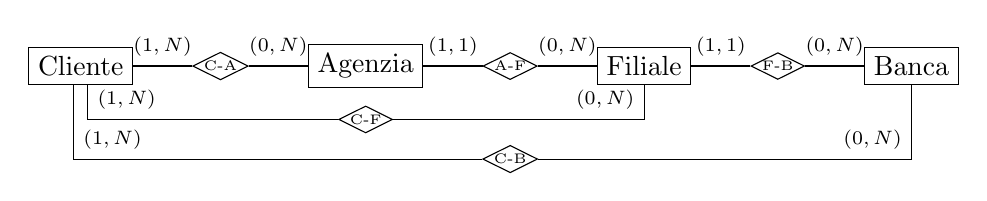
\begin{tikzpicture}
    \draw

    %%* Attributi:
    %%  node[draw, circle, inner sep=1pt, fill=black]{}node[right]{\footnotesize A}
    %%? Distanza orizzontale: E -(0.25,0.x)- A
    %%? Distanza verticale: E -(0,x * 0.22)- A

    %%* Cardinalità:
    %%  node[below right]{\scriptsize $(0,N)$}
    %%  node[above right]{\scriptsize $(0,N)$}
    %%  node[midway, above]{\scriptsize $(0,N)$}

    %%* Relazione:
    %%  node[draw, diamond, shape aspect=2, inner sep=3pt, anchor=90](r1){}
    %%  node[draw, diamond, shape aspect=2, inner sep=0.2pt, anchor=180](r1){r1}

    %%* Entità:
    %%  node[draw, rectangle, anchor=90](e1){}
    %%? Distanza verticale: E -(0.3)- R -(0.3) E
    %%? Distanza orizzontale: E -(0.75)- R -(0.75)- E
    
    (0,0)node[draw, rectangle, anchor=180](c){Cliente}
    (c.0)--++(0.75,0)node[midway, above]{\scriptsize $(1,N)$}node[draw, diamond, shape aspect=2, inner sep=0.2pt, anchor=180](r1){\tiny C-A}
    (r1.0)--++(0.75,0)node[midway, above]{\scriptsize $(0,N)$}node[draw, rectangle, anchor=180](a){Agenzia}
    (a)++(0,-0.5)node[draw, diamond, shape aspect=2, inner sep=0.2pt, anchor=90](cf){\tiny C-F}
    (a.0)--++(0.75,0)node[midway, above]{\scriptsize $(1,1)$}node[draw, diamond, shape aspect=2, inner sep=0.2pt, anchor=180](af){\tiny A-F}
    (af)++(0,-1)node[draw, diamond, shape aspect=2, inner sep=0.2pt, anchor=90](cb){\tiny C-B}
    (af.0)--++(0.75,0)node[midway, above]{\scriptsize $(0,N)$}node[draw, rectangle, anchor=180](f){Filiale}
    (f.0)--++(0.75,0)node[midway, above]{\scriptsize $(1,1)$}node[draw, diamond, shape aspect=2, inner sep=0.2pt, anchor=180](r1){\tiny F-B}
    (r1.0)--++(0.75,0)node[midway, above]{\scriptsize $(0,N)$}node[draw, rectangle, anchor=180](b){Banca}

    (c.290)|-(cf)node[midway, above right]{\scriptsize $(1,N)$}-|(f.270)node[midway, above left]{\scriptsize $(0,N)$}

    
    (c.250)|-(cb)node[midway, above right]{\scriptsize $(1,N)$}-|(b.270)node[midway, above left]{\scriptsize $(0,N)$}

    
    ;
\end{tikzpicture}
\end{document}